\subsection{Volatility Smiles 波动率微笑}

\subsubsection{简介}

\begin{itemize}
\item Volatility smiles 波动率微笑
    
    \begin{itemize}
    \item  A plot of the implied volatility of an option with a certain life as a function of its strike price (K). Volatility smiles 指期权隐含波动率 (implied volatility)与行权价格 (strike price) 之间的关系。
    
    \item  Implied volatility is volatility derived (implied) by option prices.
    \end{itemize}
    
\item The implied volatility of a European call option is the same as that of a European put option when they have the same strike price and time to maturity. 【欧式看涨期权和欧式看跌期权在具有相同行权价格和到期时间时， 其隐含波动率相同。】
    \begin{itemize}
    \item 因为波动率针对的是标的资产价格。标的资产相同，其隐含波动率也相同
    \item These results are also true to a good approximation for American options.
    \end{itemize}
    
\item 两类波动率微笑
   
    \begin{itemize}

        \item  Volatility smiles in foreign currency markets
    
        \item  Volatility smiles in equity market
    \end{itemize}
\end{itemize}


\subsubsection{2. Volatility smile for foreign currency options 外汇期权
}

\begin{itemize}
\item The implied volatility is relatively low for at-the-money (ATM) options. 【当期权是 ATM 时， 其隐含波动率最小】
    
\item It becomes progressively higher as an option moves either to in-the-money (ITM) or out-of-the-money (OTM).
    
    \begin{center}
    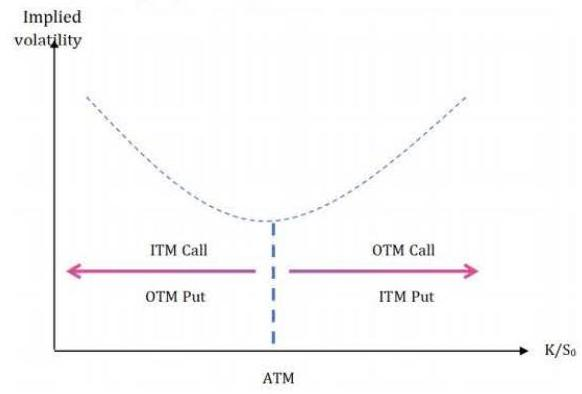
\includegraphics[width=0.4\textwidth]{images/019642cd-66db-783f-b8a5-095ec63c643b_0_531_1493_582_394_0.jpg}
    \end{center}
    \hspace*{3em} 
    
\item Implied distribution for foreign currency options
    
    \begin{itemize}
    \item Implied distribution: the risk-neutral probability distribution for an asset price at a future time from the volatility smile given by options maturing at that time.
    
    \item For foreign currency options， the implied distribution has heavier tails than the lognormal distribution with the same mean and standard deviation.【我们通常假设汇率服从对数正态分布 lognormal distribution】

    \begin{center}
    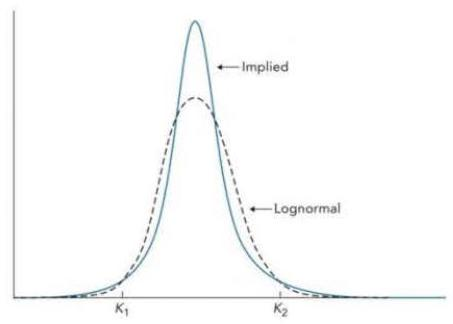
\includegraphics[width=0.3\textwidth]{images/019642cd-66db-783f-b8a5-095ec63c643b_1_603_381_453_324_0.jpg}
    \end{center}
    \hspace*{3em} 
    
    【也就是现实中， 汇率并不是服从对数正态分布。有更肥的尾部】
    
    \item 出现肥尾的原因
        \begin{itemize}
        \item 通常假设: The volatility of the asset is constant. 【实际上，汇率的波动率并不是常数】
    
        \item 通常假设: The price of the asset changes smoothly with no jumps. 【实际上， 汇率很容易出现 jump】
        \end{itemize}
    \end{itemize}
\end{itemize}




\subsubsection{Volatility smile for equity options 股票期权的隐含波动率}


\begin{itemize}
\item The implied volatility decreases as the strike price increases.
\item 股票期权的波动率微笑也叫 volatility skew.
\item The volatility used to price a low-strike-price option is significantly higher than that used to price a high-strike price option.    
    \begin{center}
    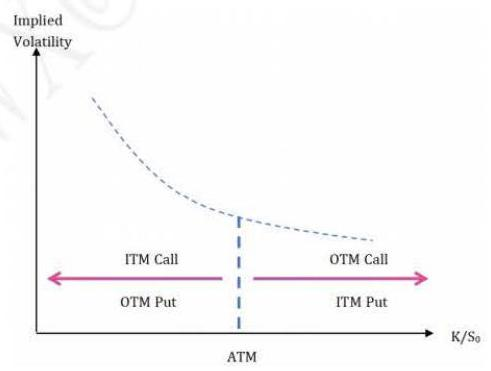
\includegraphics[width=0.4\textwidth]{images/019642cd-66db-783f-b8a5-095ec63c643b_1_579_1342_491_371_0.jpg}
    \end{center}
    \hspace*{3em} 
\item Implied distribution for equity options
    \begin{itemize}
    
        \item The implied distribution has a heavier left tail and a less heavy right tail than the lognormal distribution with the same mean and standard deviation. 【左肥右瘦】
    
    \begin{center}
    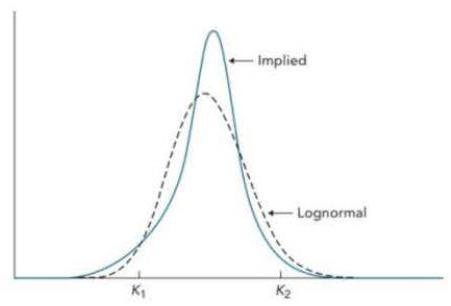
\includegraphics[width=0.3\textwidth]{images/019642cd-66db-783f-b8a5-095ec63c643b_2_598_224_451_306_0.jpg}
    \end{center}
    \hspace*{3em} 
    
    \item Reasons for the smile in equity options
        \begin{itemize}

        \item Leverage effect: as equity prices move down/up， leverage increases/decreases and as a result volatility increases/decreases.
    
        \item Volatility feedback effect: as volatility increases/decreases， investors require a higher/lower return and as a result the stock price declines/increases. 
        \item Crashophobia(崩盘效应).
        \end{itemize}
    \end{itemize}
\end{itemize}


\subsubsection{其他}

\begin{itemize}
\item 波动率微笑的其他形式:
    \begin{itemize}    
    \item 纵轴是隐含波动率，横轴是 strike price。
    \item 纵轴是隐含波动率，横轴是 \(\mathrm{K}/{\mathrm{S}}_{0}\) 。
    \item 纵轴是隐含波动率，横轴是 \(\mathrm{K}/{\mathrm{F}}_{0}\) 。
        \begin{itemize}    
        \item \({\mathrm{F}}_{0}\) : the forward price of the asset with same maturity to the option. 
        \end{itemize}
    \item 纵轴是隐含波动率，横轴是 the delta of the option。
    \end{itemize}
\item Volatility term structure
    \begin{itemize} 
    \item The relationship between the implied volatility and the time to maturity.
    \item Implied volatility tends to be an increasing function of maturity when short-dated volatilities are historically low. 【短期波动率比较低时，随着到期时间的增加， 隐含波动率上升。】
        \begin{itemize}    
        \item     预期 volatilities will increase.
        \end{itemize}
    \item Volatility tends to be a decreasing function of maturity when short-dated volatilities are historically high. 【短期波动率比较高时，随着到期时间的增加， 隐含波动率下降。】
        \begin{itemize}    
        \item     预期 volatilities will decrease.
        \end{itemize}
    \end{itemize}
\item Volatility surfaces 波动率曲面 \(\rightarrow  \mathrm{K}/{\mathrm{S}}_{0} +\) 期权到期时间
    \begin{itemize} 
    \item Volatility surfaces combine volatility smiles with the volatility term structure to tabulate the volatilities appropriate for pricing an option with any strike price and any maturity.
    
    \begin{center}
    \adjustbox{max width=\textwidth}{
    \begin{tabular}{|c|c|c|c|c|c|}
    \hline
    \multirow{2}{*}{\phantom{X}} & \multicolumn{5}{|c|}{\(\mathrm{K}/{\mathrm{S}}_{0}\)} \\
    \cline{2-6}
     & 0.90 & 0.95 & 1.00 & 1.05 & 1.10 \\
    \cline{1-6}
    1 Month & 14.2 & 13.0 & 12.0 & 13.1 & 14.5 \\
    \cline{1-6}
    3 Month & 14.0 & 13.0 & 12.0 & 13.1 & 14.2 \\
    \cline{1-6}
    6 Month & 14.1 & 13.3 & 12.5 & 13.4 & 14.3 \\
    \cline{1-6}
    1 Year & 14.7 & 14.0 & 13.5 & 14.0 & 14.8 \\
    \cline{1-6}
    2 Year & 15.0 & 14.4 & 14.0 & 14.5 & 15.1 \\
    \cline{1-6}
    5 Year & 14.8 & 14.6 & 14.4 & 14.7 & 15.0 \\
    \cline{1-6}
    \hline
    \end{tabular}
    }
    \end{center}
    \item The shape of the volatility smile depends on the option maturity. The smile tends to become less pronounced as the option maturity increases.
    \item PE 题目: A market-maker on the foreign exchange (FX) desk at an investment bank has been asked to provide a quote for an FX cal option that expires in 7 months. The option has a strike price (K) to spot price (So) ratio of 1.075. The market-maker references the following implied volatility surface when creating the quote:

    \begin{center}
    \adjustbox{max width=\textwidth}{
    \begin{tabular}{|c|c|c|c|c|c|}
    \hline
    \multirow{2}{*}{Time to expiration} & \multicolumn{5}{|c|}{Strike price to spot price ratio \(\left( {K/{S}_{0}}\right)\)} \\
    \cline{2-6}
     & 0.90 & 0.95 & 1.00 & 1.05 & 1.10 \\
    \cline{1-6}
    1 month & 9.25 & 8.55 & 8.05 & 8.70 & 9.45 \\
    \cline{1-6}
    3 months & 9.10 & 8.70 & 8.30 & 8.75 & 9.15 \\
    \cline{1-6}
    6 months & 9.45 & 9.05 & 8.70 & 9.10 & 9.45 \\
    \cline{1-6}
    1 year & 9.65 & 9.50 & 9.35 & 9.55 & 9.75 \\
    \cline{1-6}
    \hline
    \end{tabular}
    }
    \end{center}
    
    What implied volatility should the market-maker use to create the quote?
    
    A. 9.18\%
    
    B. 9.28\%
    
    C. 9.34\%
    
    D. 9.65\%
    
    Answer: C
    
    到期时间 7 个月介于 6 月和 1 年之间，要分别考虑 \(\mathrm{K}/\mathrm{S}0\) 为 1.05 和 1.10. 更具体的计算是采用线性插值法。
    

    
    \(\mathrm{K}/\mathrm{S}0 = {1.05}\) 时: \({9.10} + 1/{6}^{ * }\left( {{9.55} - {9.10}}\right)  = {9.175}\)
    
    \(\mathrm{K}/\mathrm{S}0 = {1.10}\) 时: \({9.45} + 1/{6}^{ * }\left( {{9.75} - {9.45}}\right)  = {9.5}\)
    

    
    求均值 \(= \left( {{9.175} + {9.5}}\right) /2 = {9.3375}\) .
    \end{itemize}
\item Minimum variance delta
    \begin{itemize}
    \item The formulas for delta and other Greek letters assume that the implied volatility remains the same when the asset price changes. But this is not what is usually expected to happen.
        \begin{itemize}
        \item 随着股价的波动， 隐含波动率往往会变化。这种变化导致 Delta 和其他希腊字母需要调整。
        \end{itemize}
    \item 股票价格和隐含波动率关系:
        \begin{itemize}

        \item  As the equity price increases (decreases)， \(\mathrm{K}/{\mathrm{S}}_{0}\) decreases (increases) and the volatility increases (decreases).
    
    Equity price \(\uparrow   \rightarrow  \mathrm{K}/{\mathrm{S}}_{0} \downarrow   \rightarrow\) implied volatility \(\uparrow\)
    
        \item  There is a negative correlation between equity prices and their volatilities.
    
    Equity price \(\uparrow   \rightarrow\) implied volatility \(\downarrow\)
    
        \item It turns out that the second effect dominates the first， so that implied volatilities tend to move down (up) when the equity price moves up (down). 【最终:Equity price \(\uparrow   \rightarrow\) implied volatility \(\downarrow\) 】
         \end{itemize}

    \item Minimum variance delta 最小方差 Delta:
        \begin{itemize}
        \item The delta that takes this relationship between implied volatilities and equity prices into account is referred to as the minimum variance delta.
    
        \item 最小方差 Delta 是考虑到隐含波动率和股价之间关系的调整后的 Delta。通过将隐含波动率的变化纳入期权定价模型来反映波动率和股价的关联性。
    
        \item 最小方差 Delta 通常小于传统的 Black-Scholes-Merton Delta。
        \end{itemize}
    \end{itemize}
\item Volatility frown 波动率皱眉
    \begin{itemize}
    \item 股票价格出现跳跃 Price jumps 时， 股票期权的波动率微笑会出现一种特殊的形式 \(\rightarrow\) 波动率皱眉 (volatility frown)
        \begin{itemize}
        \item 股票价格出现大幅上涨或下跌时， 这种不确定性使得隐含波动率增加， 尤其是对于 ATM 期权。
        \item 对于 OTM 和 ITM 期权，由于它们的隐含波动率取决于价格跳跃的概率假设， 其隐含波动率可能会下降。
        \end{itemize}
    \item 因此， 当出现资产价格跳跃时， 波动率微笑可能会变成一个"皱眉"。
    
    \begin{center}
    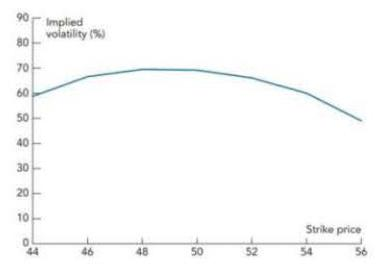
\includegraphics[width=0.3\textwidth]{images/019642cd-66db-783f-b8a5-095ec63c643b_5_634_200_376_264_0.jpg}
    \end{center}
    \hspace*{3em} 
    
    \item 具体细节【通过一个例题展示 volatility frown】
        \begin{itemize}
        \item Suppose that a stock price is currently USD 50 and an important news announcement due in a few days is expected either to increase the stock price by USD 8 or to reduce it by USD 8. The probability distribution of the stock price in， say， 1 month might then consist of a mixture of two lognormal distributions， the first corresponding to favorable news， the second to unfavorable news.
    
    \begin{center}
    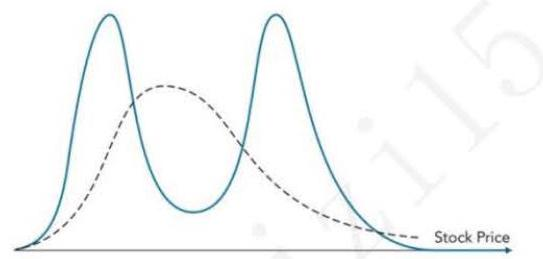
\includegraphics[width=0.4\textwidth]{images/019642cd-66db-783f-b8a5-095ec63c643b_5_590_856_543_259_0.jpg}
    \end{center}
    \hspace*{3em} 
    
    (The solid line is the true distribution; the dashed line is the lognormal distribution.)
    
    \begin{center}
    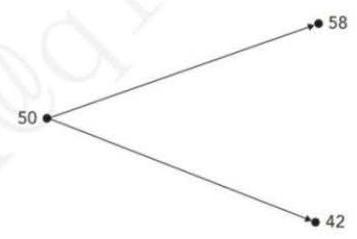
\includegraphics[width=0.3\textwidth]{images/019642cd-66db-783f-b8a5-095ec63c643b_5_660_1240_357_239_0.jpg}
    \end{center}
    \hspace*{3em} 
    
    \begin{center}
    \adjustbox{max width=\textwidth}{
    \begin{tabular}{|c|c|c|c|}
    \hline
    Strike Price (USD) & Call Price (USD) & Put Price (USD) & Implied Volatility (\%) \\
    \cline{1-4}
    42 & 8.42 & 0.00 & 0.0 \\
    \cline{1-4}
    44 & 7.37 & 0.93 & 58.8 \\
    \cline{1-4}
    46 & 6.31 & 1.86 & 66.6 \\
    \cline{1-4}
    48 & 5.26 & 2.78 & 69.5 \\
    \cline{1-4}
    50 & 4.21 & 3.71 & 69.2 \\
    \cline{1-4}
    52 & 3.16 & 4.64 & 66.1 \\
    \cline{1-4}
    54 & 2.10 & 5.57 & 60.0 \\
    \cline{1-4}
    56 & 1.05 & 6.50 & 49.0 \\
    \cline{1-4}
    58 & 0.00 & 7.42 & 0.0 \\
    \cline{1-4}
    \hline
    \end{tabular}
    }
    \end{center}
    
    (Implied Volatilities in Situation Where it is Known that the Stock Price will Move from USD 50 to Either USD 42 or USD 58 )
        \end{itemize}
    \end{itemize}
\end{itemize}


